\documentclass{article}
\usepackage{graphicx}
\usepackage{hyperref}
\usepackage{url}

\setlength{\parskip}{1em}

\begin{document}


\title{Scripting ICE with EASE}

In addition to interating with tools via the ICE user interface, ICE also
provides a scripting framework based on the Eclipse Advanced Scripting
Environment (EASE). 

\section{Installation and Configuration}

Although EASE is pre-installed in the ICE application, there are a few
additional components that need to be installed in order to provide a Python
scripting engine.

\subsection{EASE Jython Installation} 

The first step is to install the EASE Jython engine. This can be done via the
official EASE repository \href{https://dl.bintray.com/pontesegger/ease-jython/}
using the Eclipse Update Manager, but is more simply achieved using the Install
EASE Components menu.

To installed the Jython engine, select Help $\rightarrow$ Install
EASE Components in the ICE menu bar. Check the box next to the EASE Jython
Integration entry and click Finish. Follow the prompts to install the component,
and restart Eclipse when asked.

\begin{center}
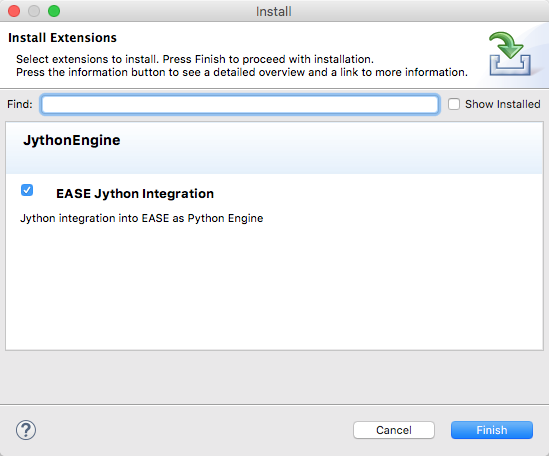
\includegraphics[width=12cm]{images/ease-marketplace}
\end{center}

\subsection{PyDev Installation (optional)} 

It is possible to edit Python scripts in Eclipse using the default text editor,
however it is much more productive to use the PyDev Eclipse development
environment. In addition to the usual syntax coloring and other advanced editing
features you'd expect in Eclipse, PyDev also provides the ability to run and
debug Python programs from within the Eclipse environment.

PyDev can be easily installed from using the Eclipse Marketplace client as
follows. From the ICE menu bar, select Help $\rightarrow$ Eclipse
Marketplace\ldots, type ``pydev'' in the Find field, then click the Go button.
After a few seconds, you should see an entry for PyDev. Simply click the Install
button and follow the prompts to install the feature. Once Eclipse has been
restarted, any Python scripts ending in ``.py'' will be recognised by
PyDev and opened in the Python editor by default.

\begin{center}
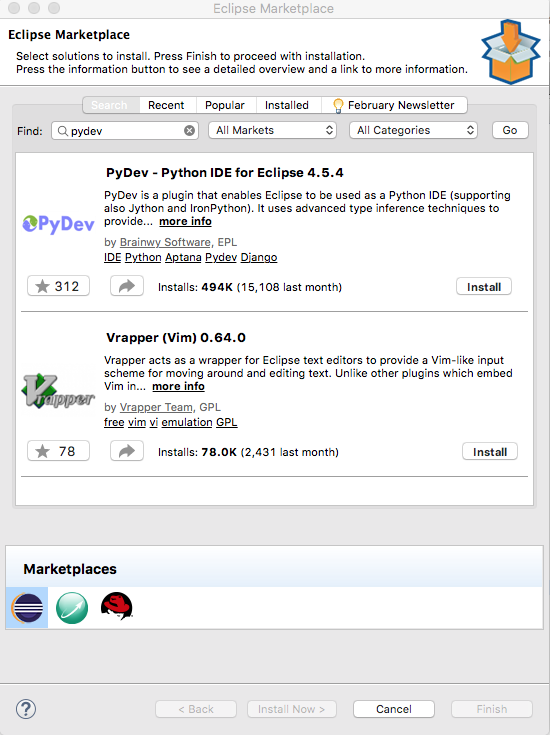
\includegraphics[width=12cm]{images/pydev-marketplace}
\end{center}

\subsection{EASE Configuration}

By default, EASE is configured to use the javascript (Rhino) engine. Since this
tutorial assumes that the preferred environment is Python, we recommend changing
this default. This is done through the Scripting preferences.

To set the script engine default, select Window $\rightarrow$ Preferences\ldots
in the ICE menu bar. (On Mac OS X, Preferences\ldots is instead located under
Eclipse ICE in the menu bar.) Open the Scripting tree item on the left side of
the Preferences window, then select Shell. Select ``Python (Jython)'' from the
Preferred Engine dropdown, then click on OK.

\begin{center}
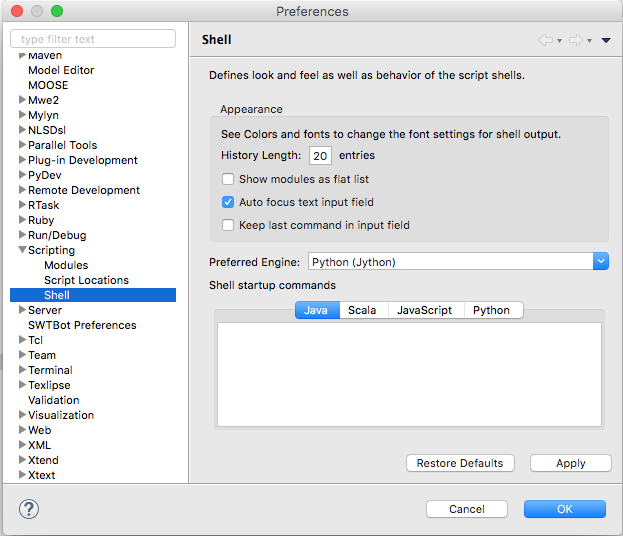
\includegraphics[width=12cm]{images/scripting-prefs}
\end{center}

\section{Creating and Running Scripts}

EASE provides a perspective for creating, managing, debugging, and running
scripts. However for the purposes of this tutorial, we will create the scripts
using PyDev and run them directly.

\subsection{Creating a Python Script}

The easiest way to create a Python script is to simply create a text file ending
in ``.py'' in an existing project. If your scripts will be used with stand-alone Python
programs, you can use PyDev to create a Python project, but in general, any kind
of project will suffice.

\subsection{Running a Python Script}

Once you have created Python script, is can be easily launched using the Run As
context menu. Simply right-click on the Python file, then select Run As
$\rightarrow$ EASE Script. EASE will automatically recognize the file type and
run the script with the appropriate engine. Any (textual) output generated by
the script will be displayed in the Console view.

\section{Using the Sample Scripts}

Four samples scripts are available to show how ICE can be scripted using EASE.
These scripts can be obtained by cloning the ICE Git repository from
\href{https://github.com/eclipse/ice.git}, then importing the
org.eclipse.ice.examples.reflectivity package into your workspace. Once you've
completed this, you should see the following scripts:

\textbf{createAndEditPython.py:} This script demonstrates\ldots

\textbf{createAndProcessPython.py:} This script demonstrates\ldots

\textbf{iterateChangeParameterPython.py:} This script demonstrates\ldots

\textbf{listFromScratchPython.py:} This script demonstrates\ldots

\section{Writing Python Scripts}

EASE hides many of the details that would normally be required to manipulate
Java objects and perform actions in the Eclipse IDE. It does this by
encapsulating typical actions into simple script commands that can be easily
invoked from scripts that you write.

See the EASE documentation \href{http://eclipse.org/ease/documentation} for more information on developing EASE scripts.

\end{document}
